% Generated by functionality.generate_paper_replots().
\begin{figure}[!htbp]
\centering
\begin{minipage}{0.49\textwidth}
\centering
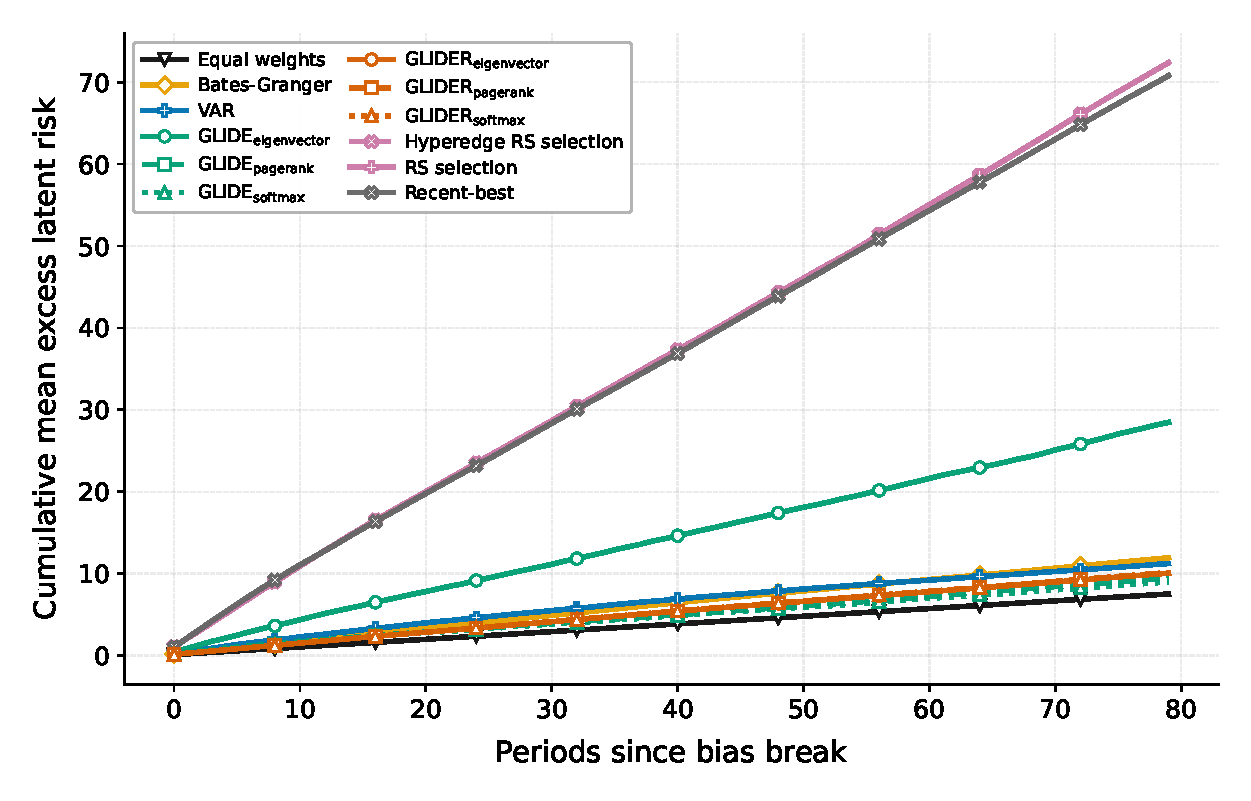
\includegraphics[width=\linewidth]{Empirical_Data/empirical_outputs/paper_replots/adaptability_ier_2A.pdf}
\end{minipage}\hfill
\begin{minipage}{0.49\textwidth}
\centering
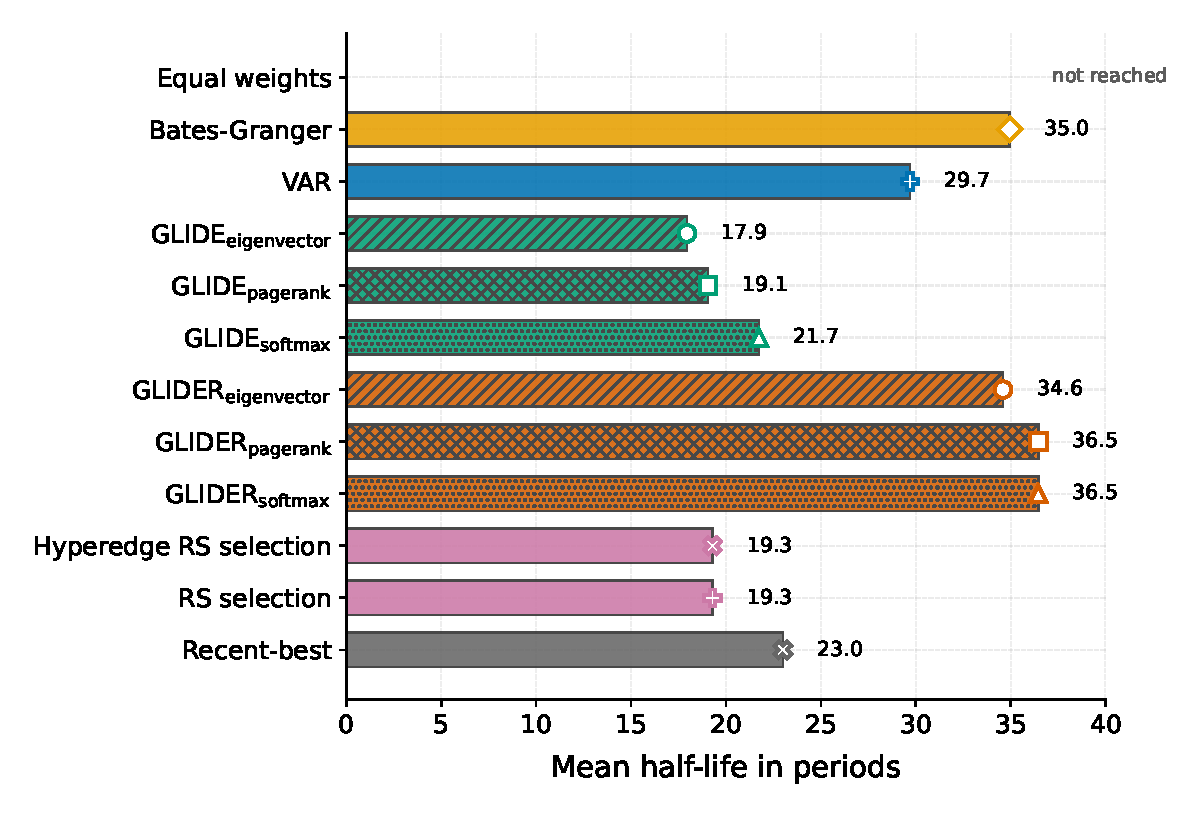
\includegraphics[width=\linewidth]{Empirical_Data/empirical_outputs/paper_replots/adaptability_half_life_2A.pdf}
\end{minipage}
\vspace{0.5em}
\begin{minipage}{0.49\textwidth}
\centering
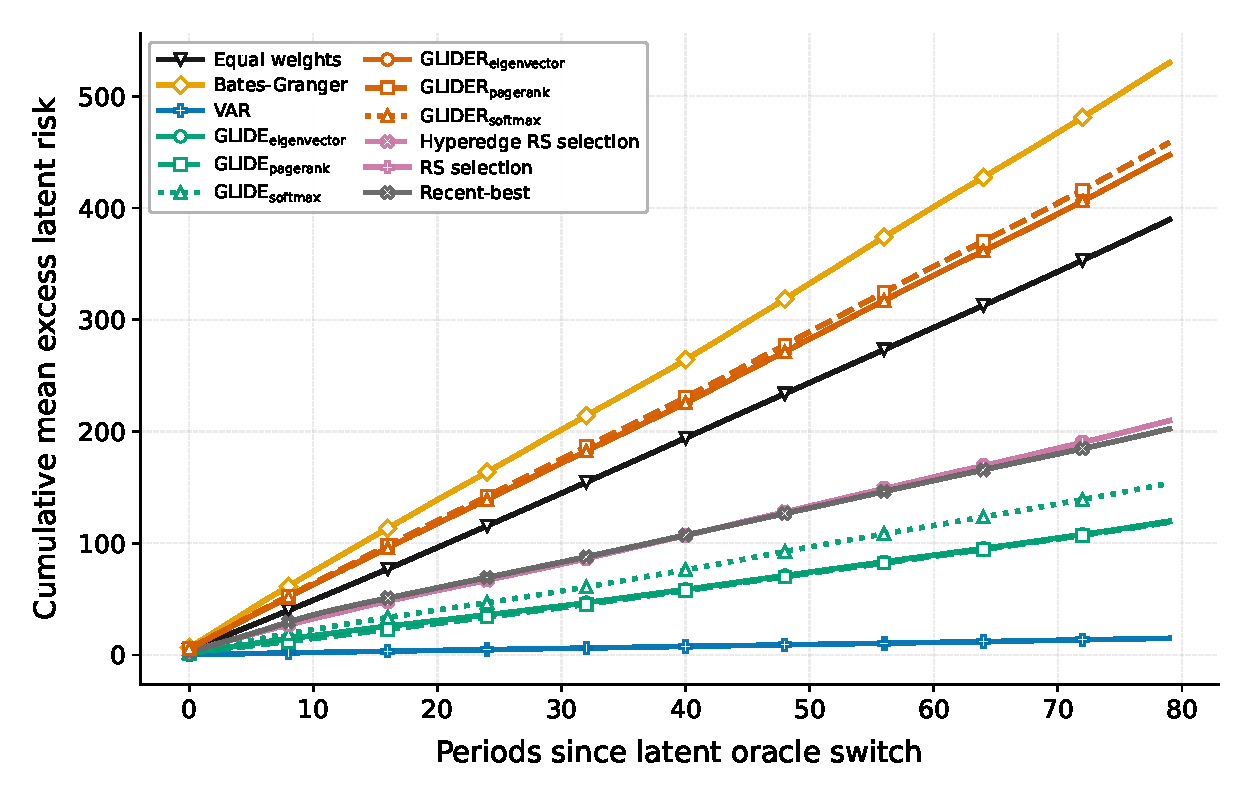
\includegraphics[width=\linewidth]{Empirical_Data/empirical_outputs/paper_replots/adaptability_ier_2B.pdf}
\end{minipage}\hfill
\begin{minipage}{0.49\textwidth}
\centering
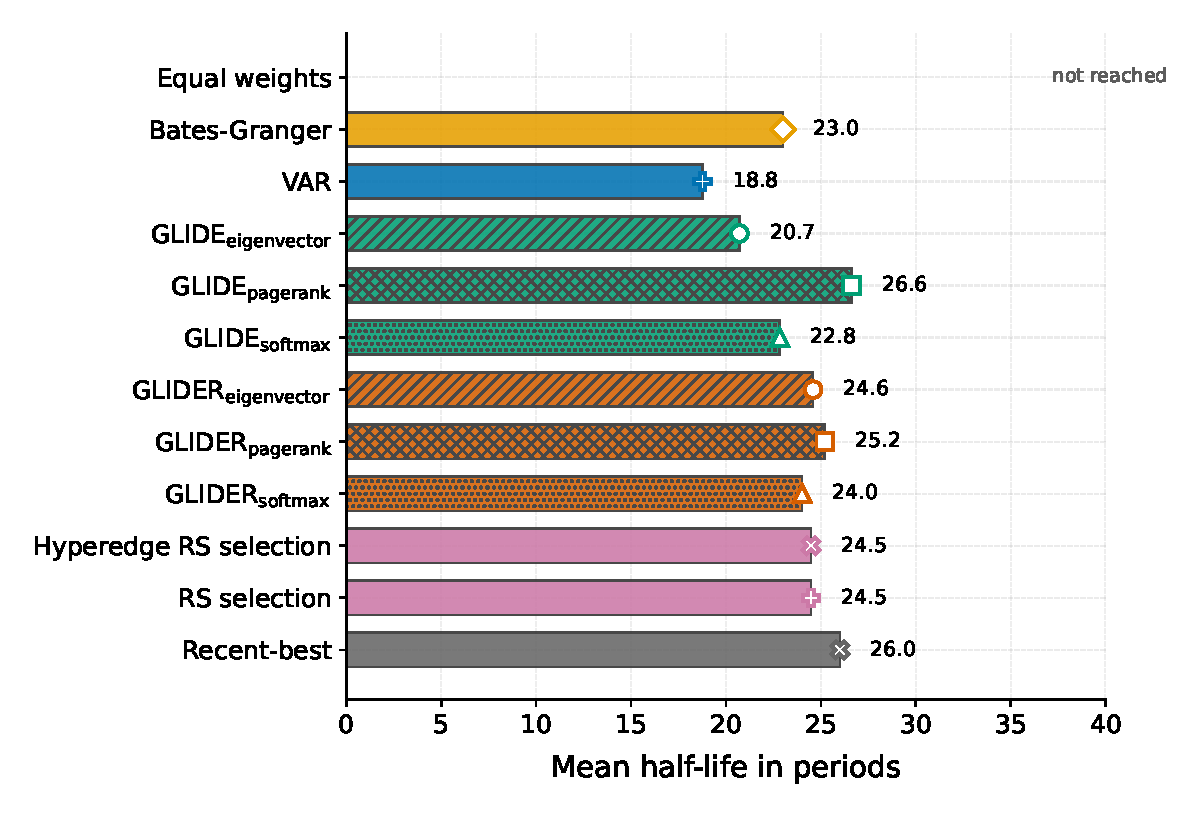
\includegraphics[width=\linewidth]{Empirical_Data/empirical_outputs/paper_replots/adaptability_half_life_2B.pdf}
\end{minipage}
\caption{Adaptability diagnostics for Scenarios 2A and 2B. Scenario 2A is measured at the known bias break across multiple simulation replications; Scenario 2B is measured on full-window latent-oracle switch events across multiple simulation replications. Left panels show cumulative sums of mean excess latent risk, so near-linear curves reflect nearly constant horizon-level excess risk rather than a linear recovery path; right panels show mean half-life, where lower values indicate faster adaptation and not-reached entries are undefined within the event window rather than zero.}
\label{fig:adaptability-side-by-side}
\end{figure}
